\chapter{Result and Output}

\section{Result and Discussion}
We have implemented the project as a full stack Invoice Web Application with a convenient user interface focusing on ease of use for all the users since it is implemented as a general-purpose application common for any user.  

The system specifications such as User Login and Authentication, Invoice Dashboard and Invoice History, Create Invoices, Update and Delete Invoices, Generate Invoice PDF are meet while developing the system design.

The system design is developed considering the specification and requirements which is clearly representing the interfaces needed to be developed in application.

The web application is designed accordingly to the interfaces specified in the system design.This web application is implemented using the technologies such as basic web components involving html, css, javascript and php. Also, we have used few web api's required to implement the invoice as pdf and mail those invoice pdf to the customers. Frameworks based on css and javascript are used to implement some functionalities wherever required. 

Development tools like dompdf is used to implement pdf generation of the invoices.

\section{Output}

\subsection{Authentication}

\begin{figure}[h]\centering
	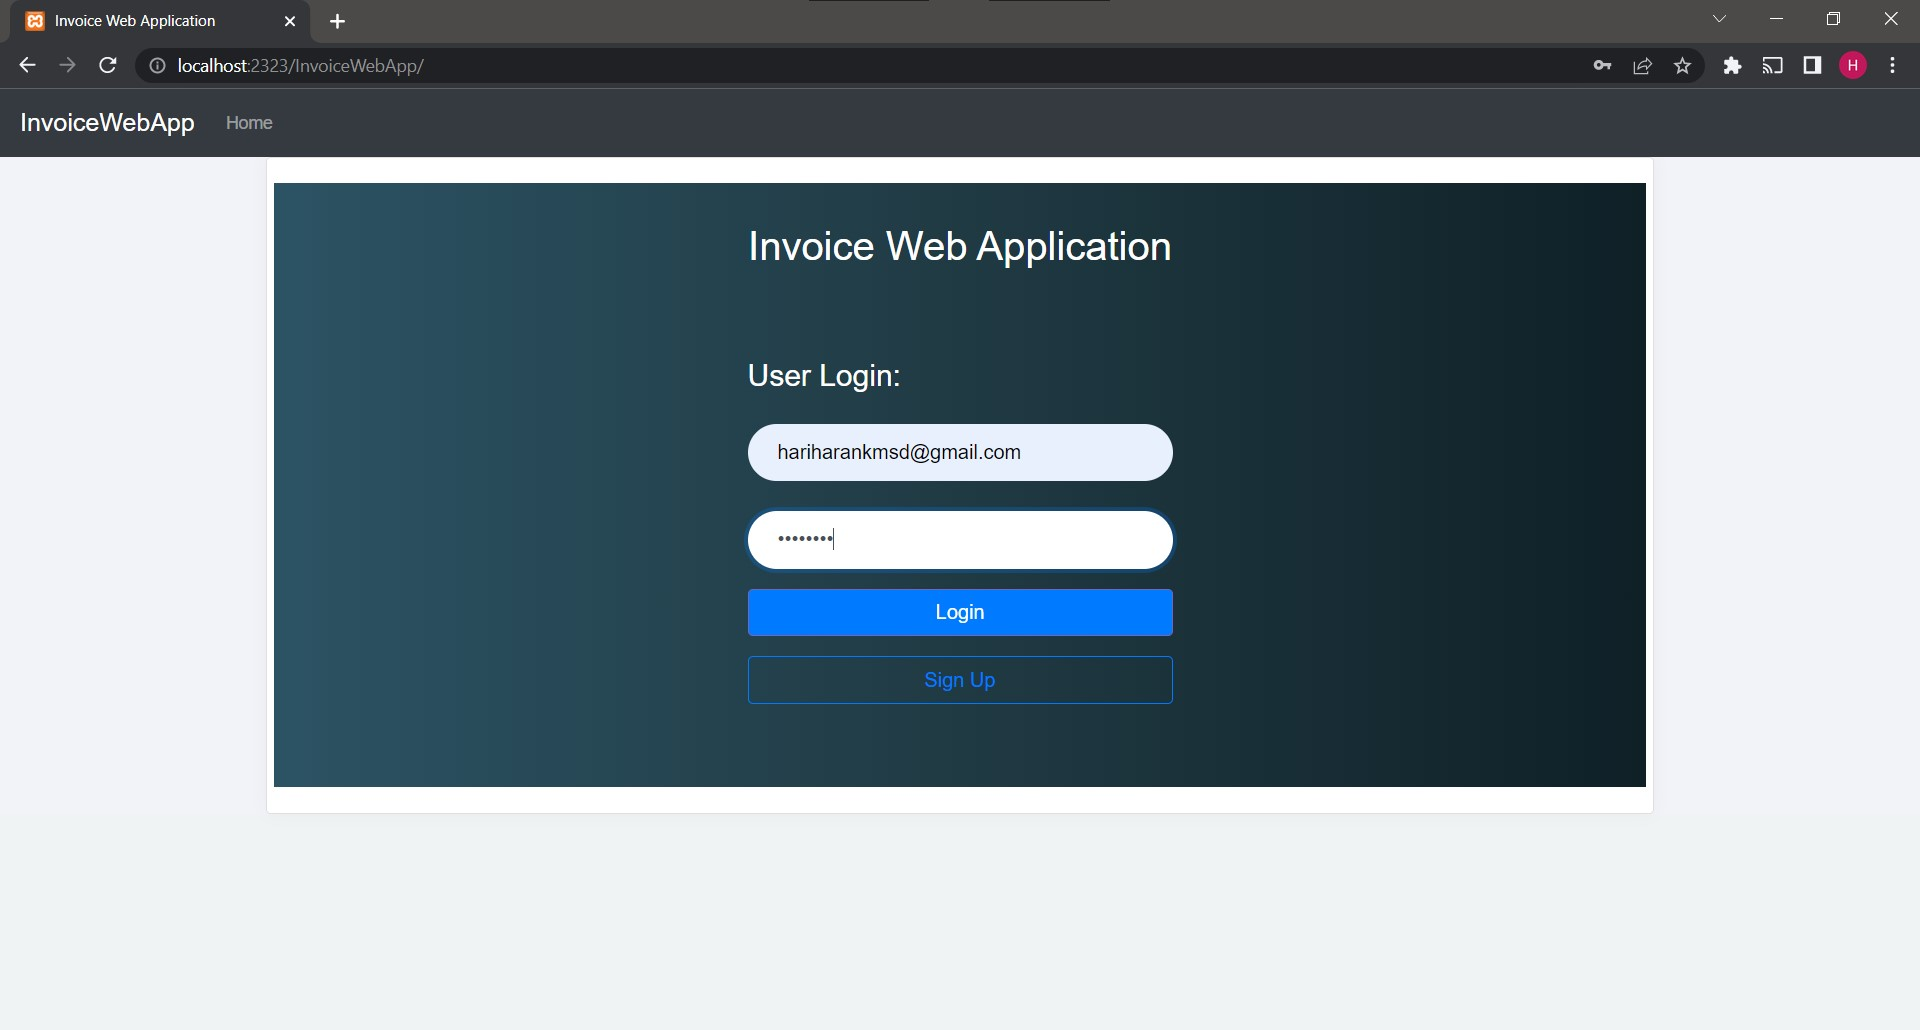
\includegraphics[width=6in]{./images/login.jpg}
	\caption{User Login Authentication Interface}\label{login}
\end{figure}



\begin{figure}[h]\centering
	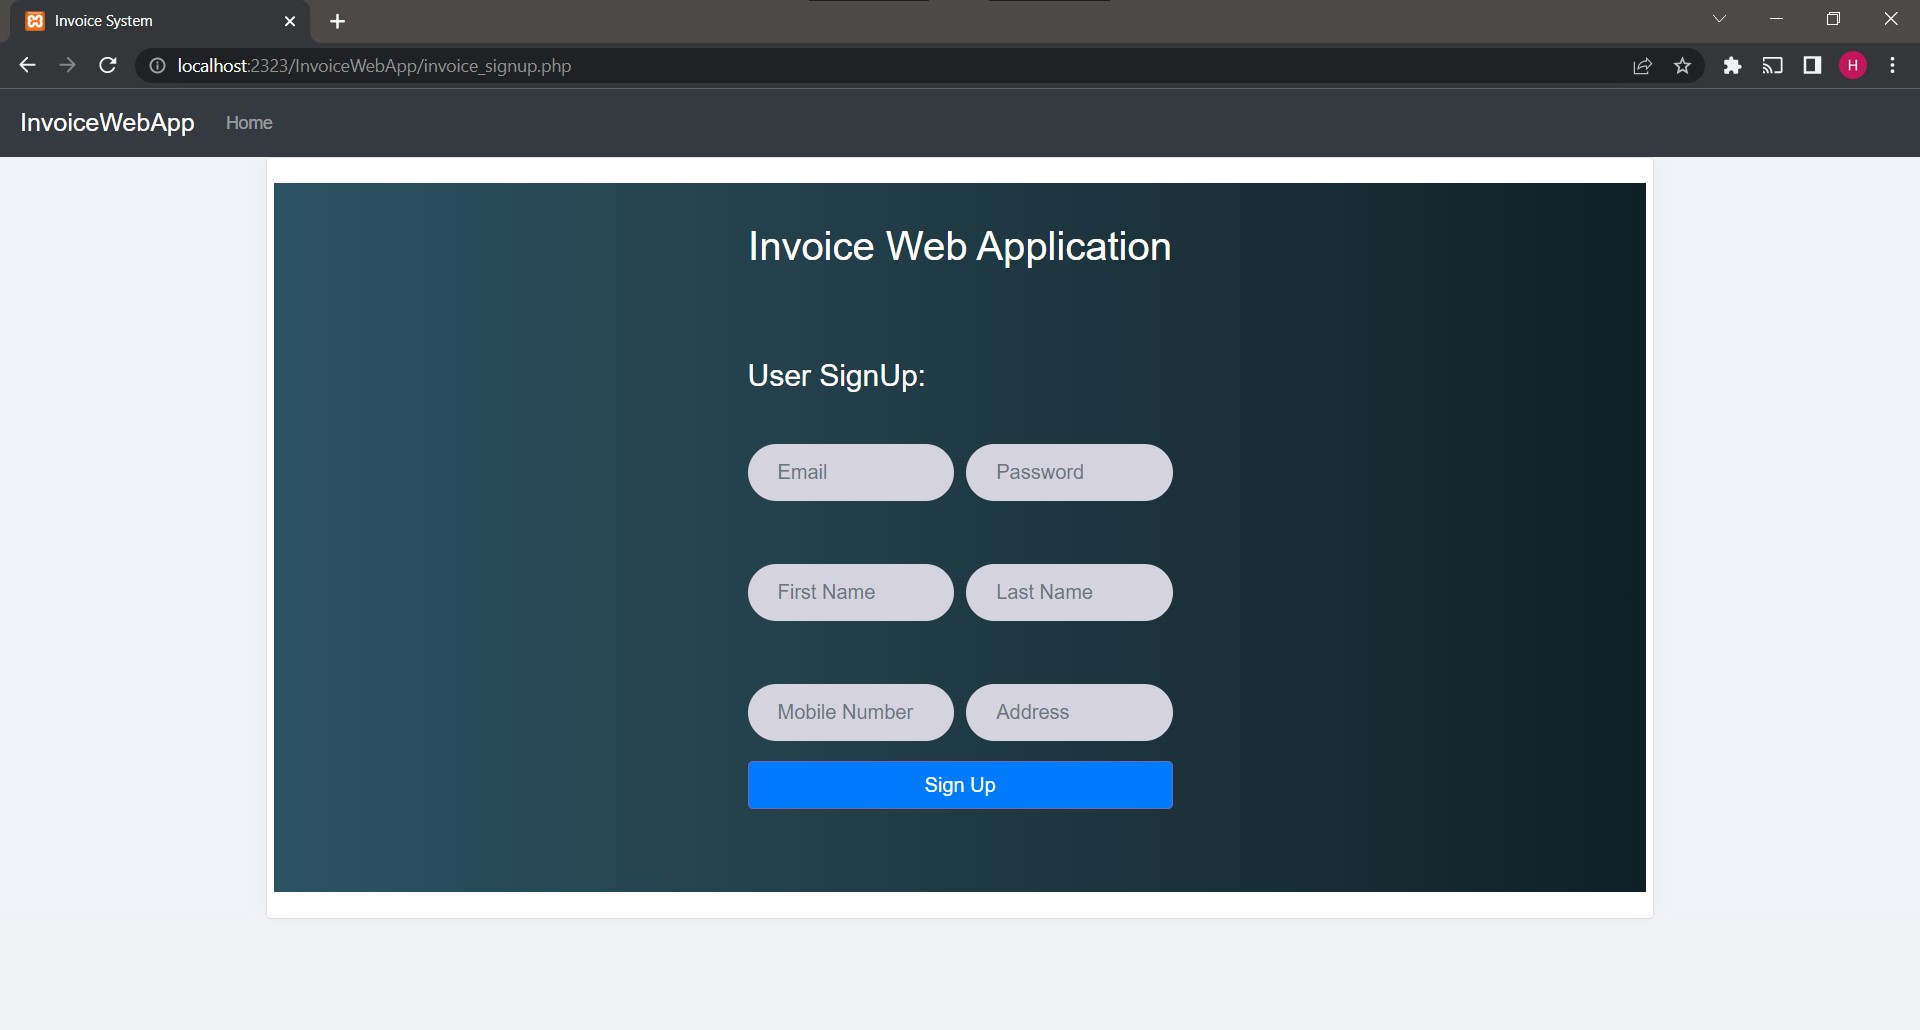
\includegraphics[width=6in]{./images/signup.jpg}
	\caption{Sign Up Interface for profile creation}\label{signup}
\end{figure}

\pagebreak

\subsection{User Interface}
\begin{figure}[h]\centering
	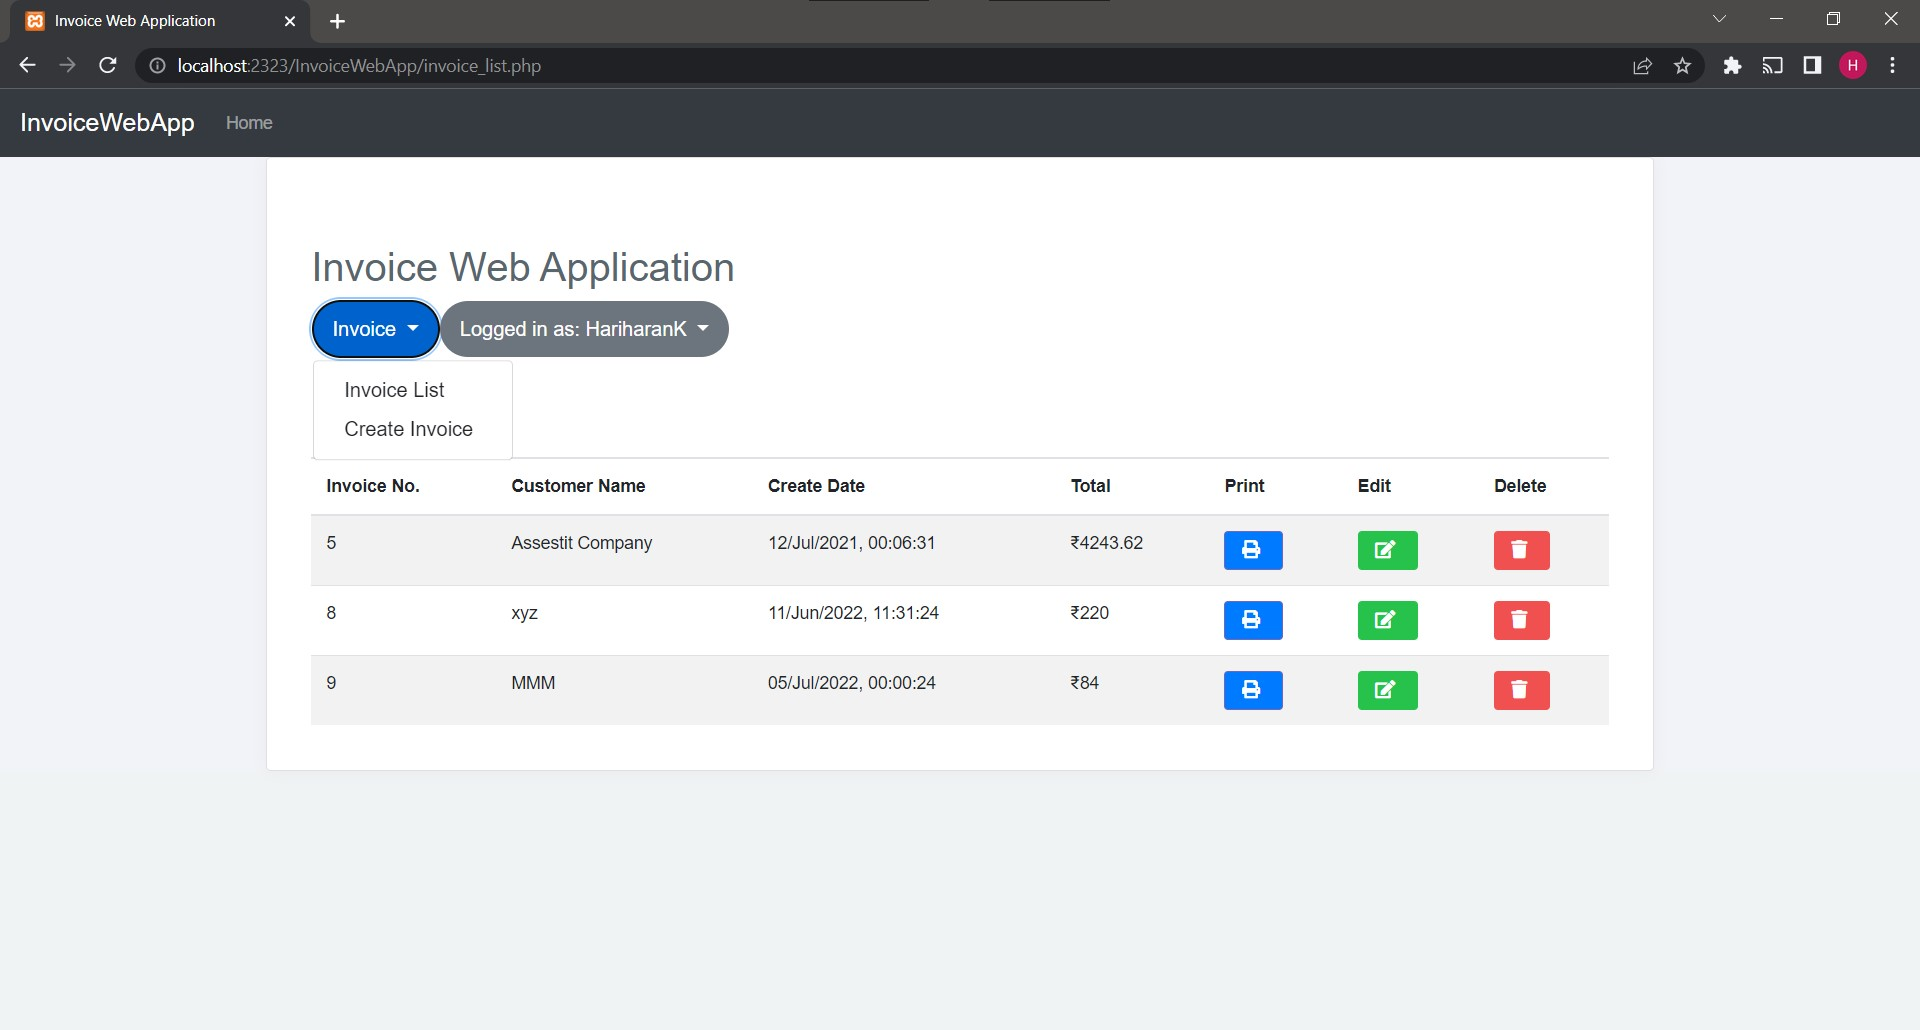
\includegraphics[width=6in]{./images/dashboard.jpg}
	\caption{Dashboard with Invoices list. Access to all other interfaces}\label{dashboard}
\end{figure}

\begin{figure}[h]\centering
	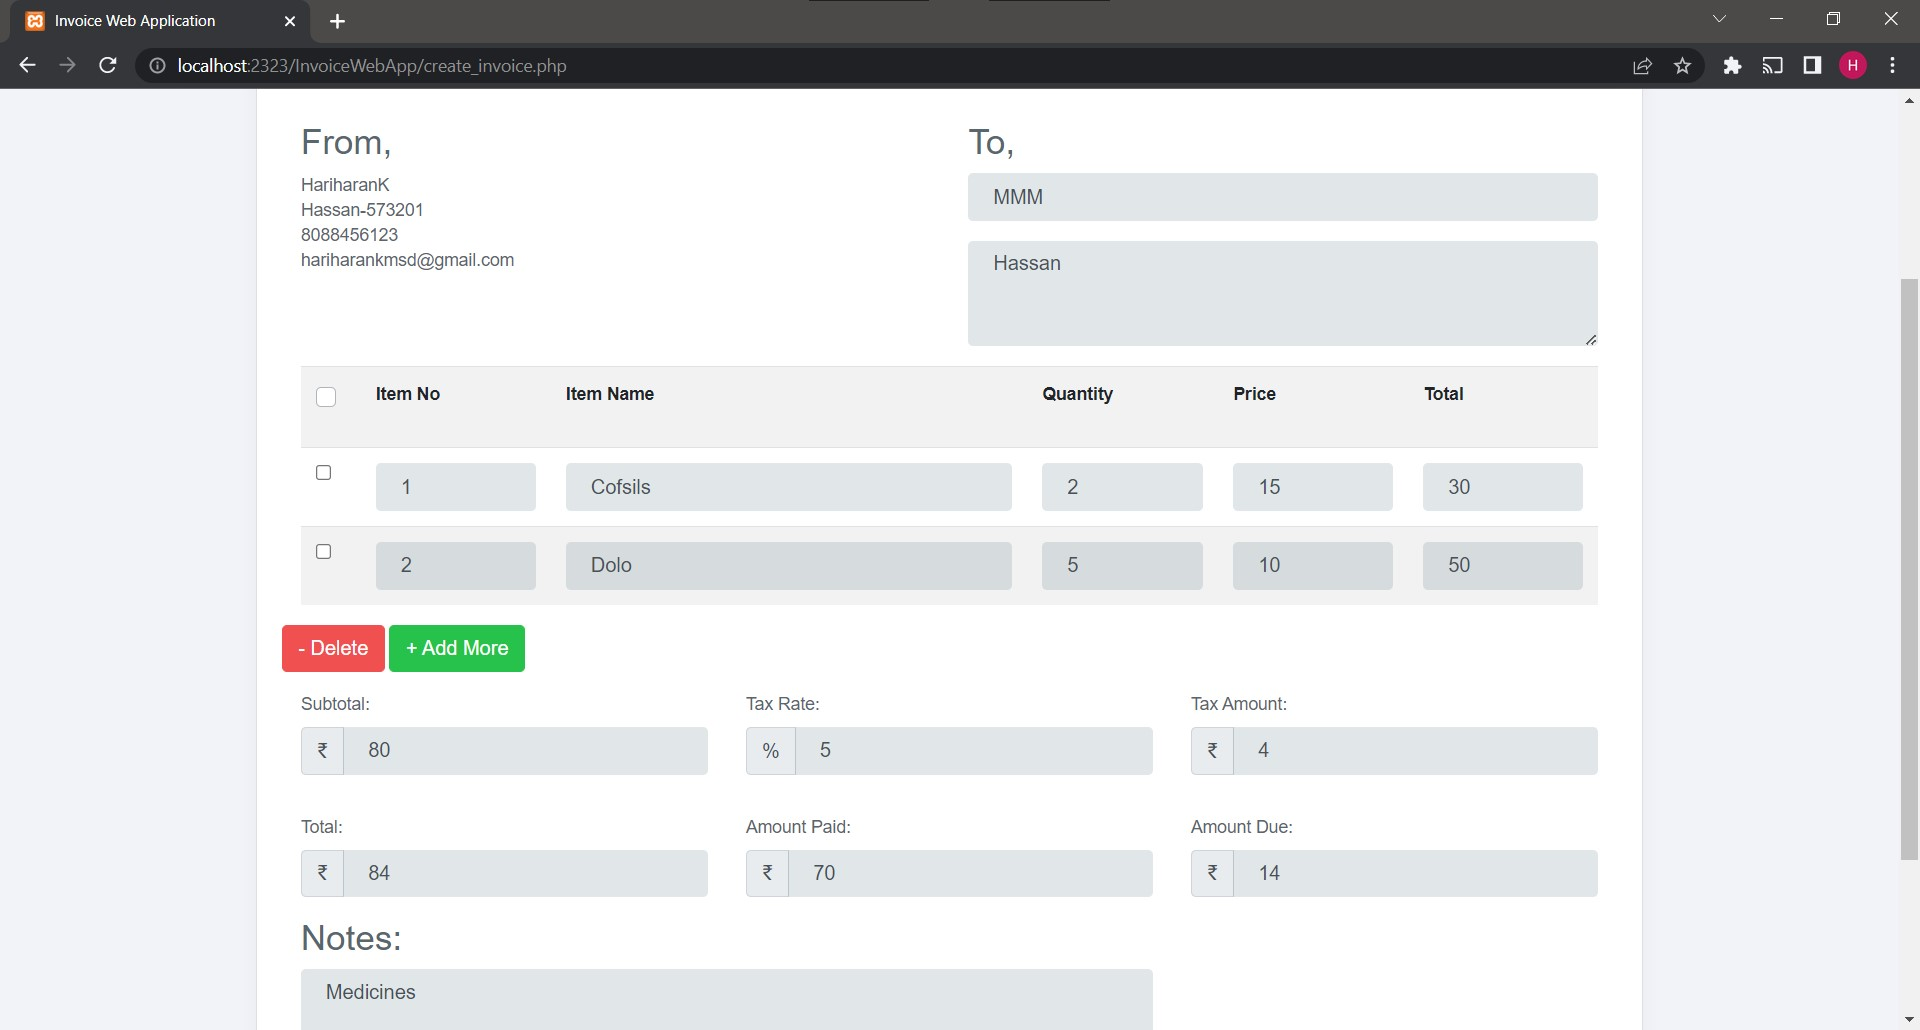
\includegraphics[width=6in]{./images/createInvoice.jpg}
	\caption{Create new invoice interface}\label{createInvoice}
\end{figure}

\pagebreak

\begin{figure}[h]\centering
	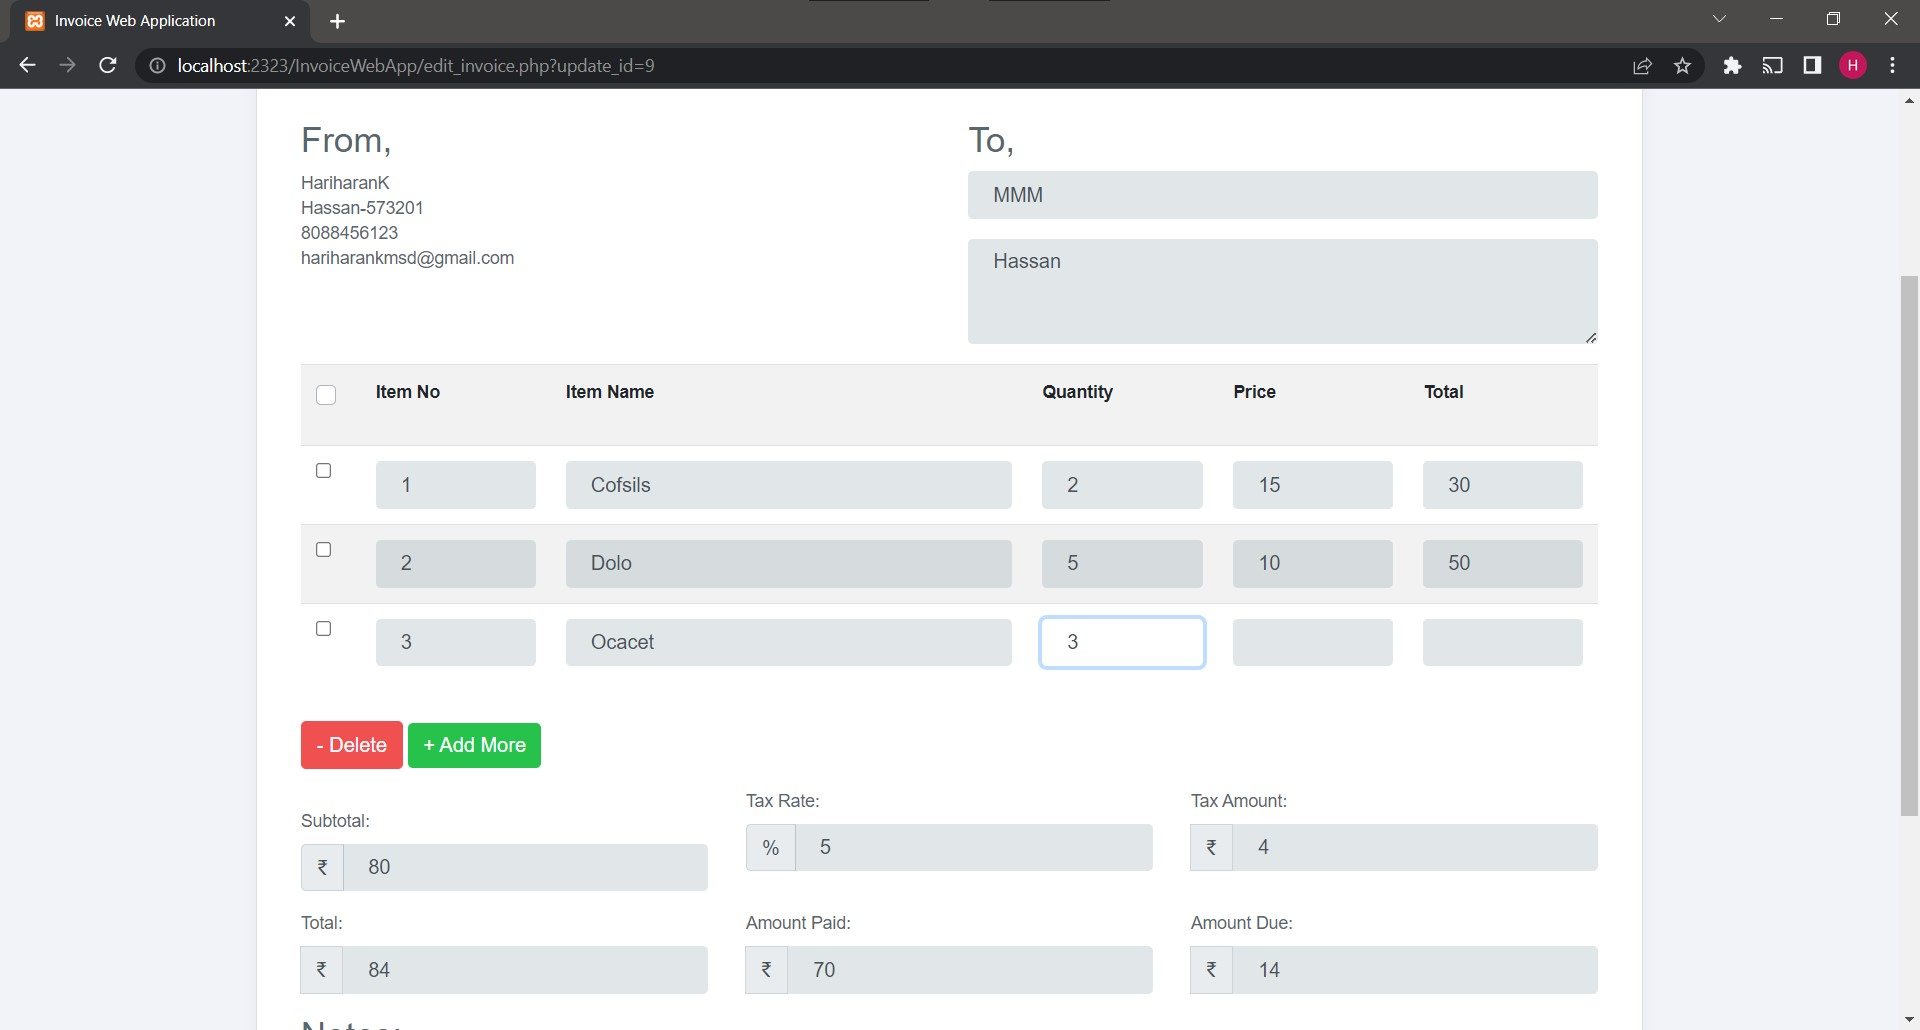
\includegraphics[width=6in]{./images/editInvoice.jpg}
	\caption{Edit existing invoices and Update the Invoice}\label{editInvoice}
\end{figure}

\begin{figure}[h]\centering
	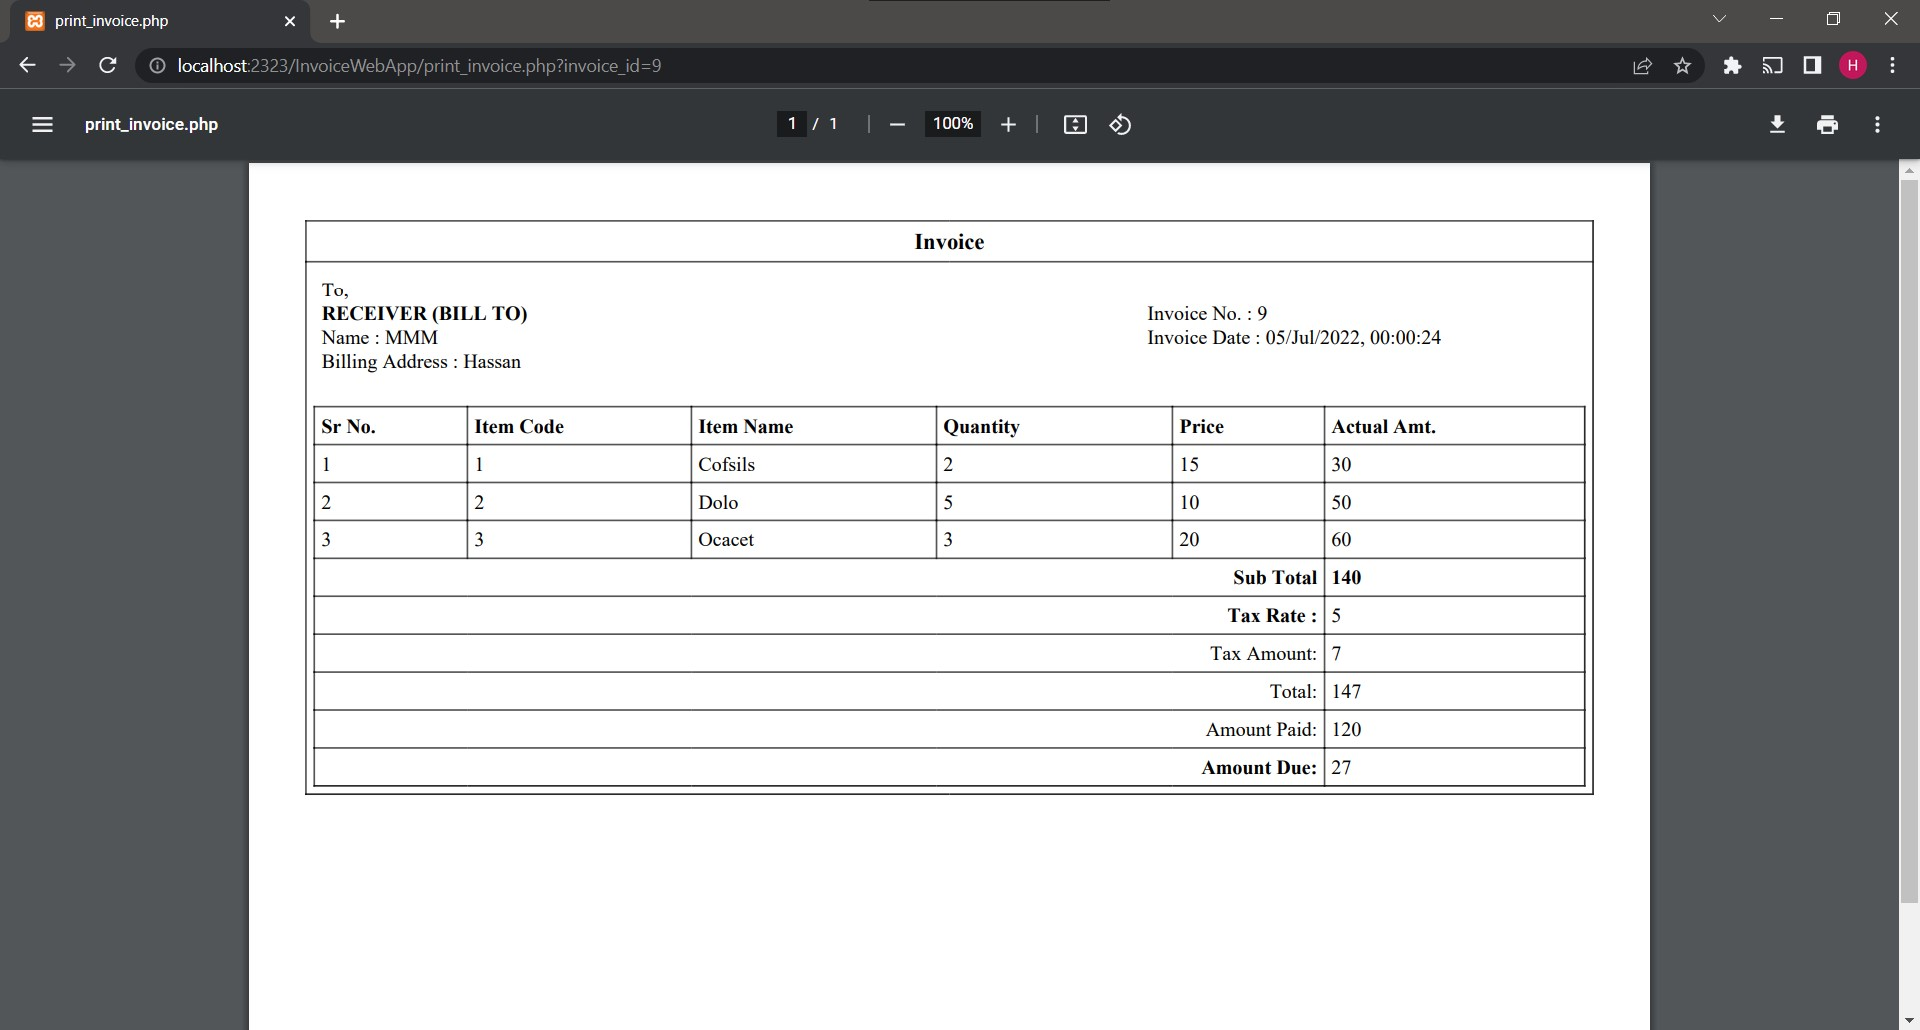
\includegraphics[width=6in]{./images/printInvoice.jpg}
	\caption{Print the invoice from generated invoice PDF}\label{printInvoice}
\end{figure}

\pagebreak

\subsection{Database Tables}

Tables list in database
\begin{table}[h]\centering
	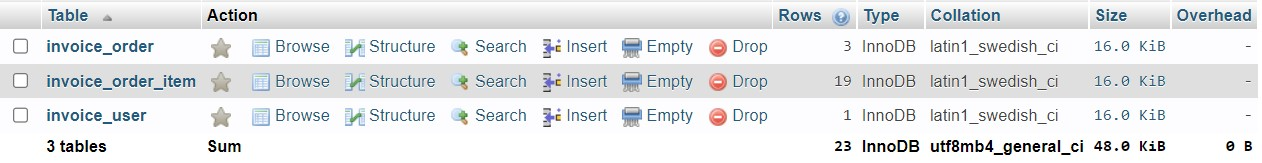
\includegraphics[width=6in]{./images/invoicetables.jpg}
	\caption{List of tables in the database}\label{invoicetables}
\end{table}

Database tables with entries 
\begin{table}[h]\centering  
    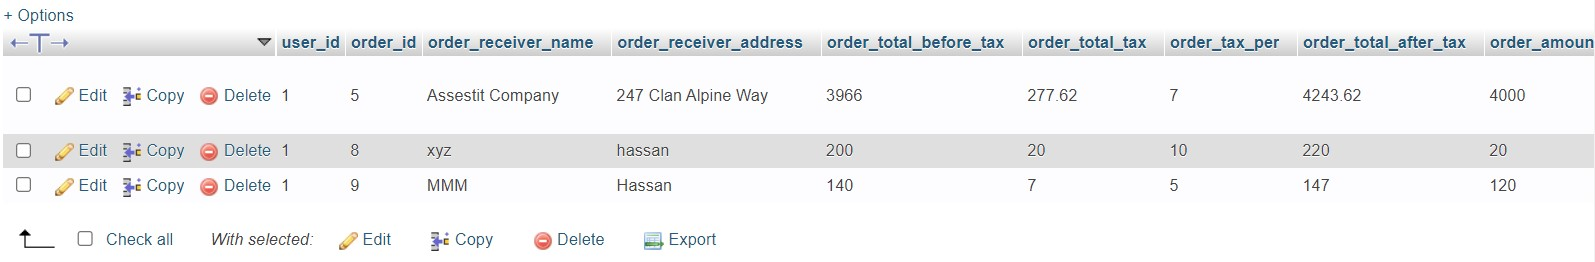
\includegraphics[width=6in]{./images/invoiceorder.jpg}
	\caption{Invoice Order table: details of each order}\label{invoiceorder}
	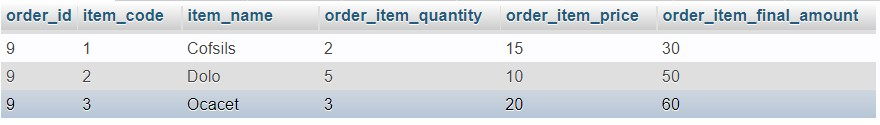
\includegraphics[width=6in]{./images/invoiceorderitem.jpg}
	\caption{Invoice Order Items table: details of items in each order}\label{invoiceorderitem}
	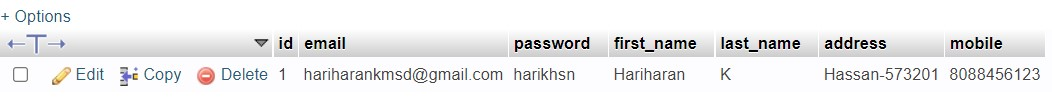
\includegraphics[width=6in]{./images/invoiceuser.jpg}
	\caption{Invoice Users table: details of user profiles}\label{invoiceuser}
\end{table}

% \begin{figure}[h]\centering
%     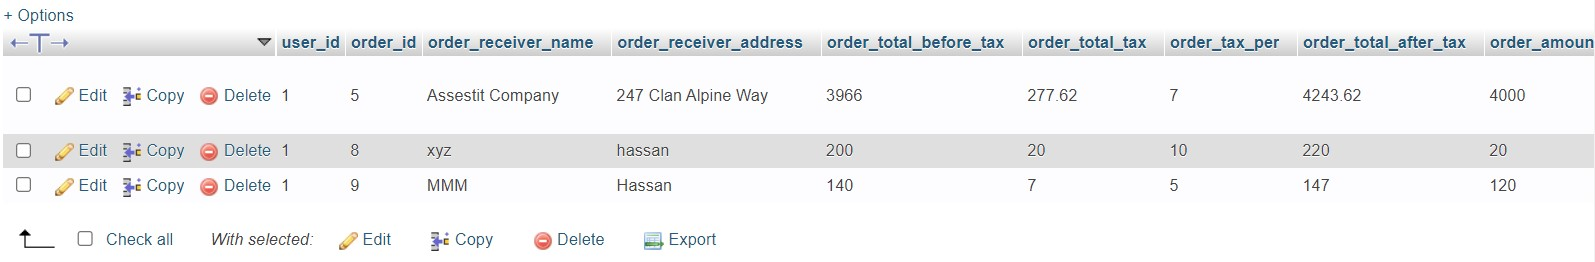
\includegraphics[width=6in]{./images/invoiceorder.jpg}
% 	\caption{Print the invoice from generated invoice PDF}\label{invoiceorder}
% 	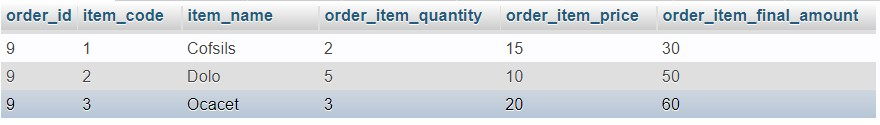
\includegraphics[width=6in]{./images/invoiceorderitem.jpg}
% 	\caption{Print the invoice from generated invoice PDF}\label{invoiceorderitem}
% 	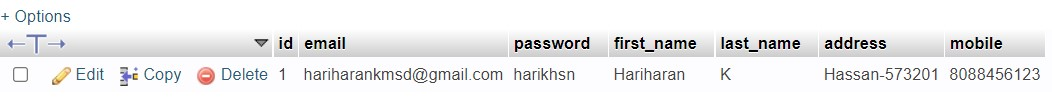
\includegraphics[width=6in]{./images/invoiceuser.jpg}
% 	\caption{Print the invoice from generated invoice PDF}\label{invoiceuser}
% \end{figure}
% \caption{Comparison of Community Detection Algorithms}\label{comp}